% Working report based on the supplied DA241O final term paper template.
% Overleaf main document: main.tex. Build with pdfLaTeX, Biber, then pdfLaTeX twice.
% Unfinished sections retain the template's instructional placeholders.
% The explicit page breaks before References and the back matter reproduce
% the supplied template; remove/adapt those breaks when writing the report.
\documentclass[12pt,a4paper]{article}
\usepackage[T1]{fontenc}
% Latin Modern follows the Computer Modern typography of Assignments 1 and 2.
\usepackage{lmodern}
\usepackage{microtype}
\usepackage{graphicx}
\usepackage[section]{placeins}
\usepackage{caption}
\usepackage{booktabs}
\usepackage{array}
\usepackage{amsmath}
\usepackage{csquotes}
\usepackage[backend=biber,style=apa,sorting=nyt]{biblatex}
\addbibresource{airline_references.bib}
\captionsetup[figure]{font=small,labelfont=bf,justification=raggedright,singlelinecheck=false,skip=7pt}
\usepackage[margin=1in]{geometry}
\usepackage{setspace}
\onehalfspacing
\setlength{\parindent}{0pt}
\setlength{\parskip}{6pt}
\usepackage{titlesec}
\titleformat{\section}{\large\bfseries}{\thesection.}{0.6em}{}
\titleformat{\subsection}{\normalsize\bfseries}{\thesubsection}{0.6em}{}
\titlespacing*{\section}{0pt}{1.2em}{0.45em}
\titlespacing*{\subsection}{0pt}{0.85em}{0.3em}
\usepackage{fancyhdr}
\pagestyle{fancy}
\fancyhf{}
\fancyhead[L]{DA241O: Managerial Economics}
\fancyhead[R]{Final Term Paper}
\fancyfoot[C]{\thepage}
\renewcommand{\headrulewidth}{0.4pt}
\setlength{\headheight}{14.5pt}
\addtolength{\headsep}{-2.5pt}
\usepackage[hidelinks]{hyperref}

% The source prints its bullets as ordinary, unindented paragraphs.
\newcommand{\templatebullet}[1]{\par\noindent\textbullet\hspace{5.88pt}#1\par}

\begin{document}
\hypersetup{pageanchor=false}
\begin{titlepage}
\centering
\vspace*{1cm}
{\Large\bfseries DA241O: MANAGERIAL ECONOMICS\par}
\vspace{0.8cm}
{\LARGE\bfseries Final Term Paper\par}
\vspace{1cm}
{\Large\bfseries From Fragmentation to Duopoly: Market Concentration and Major Consolidation Events in Indian Domestic Aviation between 2015--2026\par}
\vspace{1cm}
{\large\textbf{Team Name:} Macro Matrix\par}
{\large\textbf{Team No.:} 8\par}
\vspace{0.75cm}
{\large\textbf{Team Members:}\par}
\vspace{0.3cm}
{\large Goutham P\\
Meena Chidambaram\\
Sowmya K\\
Sweta Behera\par}
\vfill
{\large M.Tech in AI\\
Indian Institute of Science\\[0.5cm]
\textbf{Submission Date:} 20th November 2026\par}
\end{titlepage}
\hypersetup{pageanchor=true}
\setcounter{page}{1}

\section*{Abstract}
Briefly present the research problem, research question, data and methodology, main findings, and key implications.

\vspace{0.5cm}
\textbf{Keywords:} [Keyword 1]; [Keyword 2]; [Keyword 3]; [Keyword 4]

\section{Introduction}
\subsection{Background and Problem Statement}
Introduce the market, firm, sector, or policy setting being studied and explain the problem being investigated.

\subsection{Research Question}
State the primary research question.

\subsection{Research Objectives}
State the 2--3 research objectives.

\subsection{Economic Framework}
Identify the economic concept or framework used in the study and explain its relevance to the research question.

Examples may include demand and supply, market structure, information asymmetry, adverse selection, network effects, opportunity cost, principal-agent problems, or other relevant concepts from the course.

\subsection{Scope of the Study}
Specify the relevant market, geography, time period, population, firms, products, or other boundaries of the study.

\section{Literature Review}
\subsection{Existing Literature}
Review the relevant academic, government, industry, and other credible sources.

\subsection{Synthesis of Literature}
Discuss the major findings, patterns, and differences across the literature.

\subsection{Research Gap}
Clearly identify what is not adequately addressed by the existing literature and how the present study addresses this gap.

\subsection{Relevance to the Present Study}
Explain how the existing literature and identified gap inform the research question and analysis.

\section{Data and Methodology}
\subsection{Research Design}
Briefly describe the research design used in the study.

\subsection{Data Sources}
Describe the data source or sources, period covered, geographic coverage, sample or number of observations where applicable, and data collection procedure where applicable.

\subsection{Unit of Analysis}
Clearly identify the unit of analysis, such as firm, product, transaction, household, district, city, industry, or another relevant unit.

\subsection{Variables and Measures}
Define the key variables, indicators, measures, or categories used in the analysis.

For quantitative studies, identify the dependent variable, main explanatory variables, and relevant control variables where applicable.

\textbf{O4.} Appendix~\ref{app:o4-dictionary} defines the inputs, constructed measures, units, sample flags and source-quality conventions used in the concentration and buffer calculations.

\clearpage
\subsection{Method of Analysis}
\textbf{O4.} Descriptive index and comparative analysis assess two-group dominance and dependence on IndiGo. Each month's national passenger counts and route scheduled-flight counts are aggregated into ownership groups and ranked to calculate HHI, CR2, the leader--rival share gap and fringe share, with the leading groups identified. Route shares pool both directions of the twenty busiest airport pairs by 2025 passengers. The predefined flags are CR2 $\geq80\%$, fringe $\leq20\%$ and gap $>20$ pp, with HHI $>1{,}800$ used as a high-concentration benchmark \parencite[Section~2.1]{dojftc2023merger}. The gap and the IndiGo $\geq60\%$ frequency-share flag are study-defined; monthly exposure percentages use available pairs as their denominator, with IndiGo-only observations identified separately. Rivals' unused capacity is summed as ASK minus RPK and expressed as a percentage of IndiGo's RPK for December 2024 and December 2025. A matched December 2024--July 2026 comparison includes the top-ten subset, while H6 retains the full available April 2019--September 2026 route panel. Missing observations are excluded. Appendix~\ref{app:o4-route-preparation} records ownership conventions, source-quality checks, exclusions and worked calculations.

\subsection{Hypotheses or Expected Relationships}
\textbf{H5 (O4): National concentration.} We expect IndiGo and the Air India Group to remain the two largest groups in every month from December 2024 to July 2026, with CR2 $\geq80\%$ and a share gap above 20 percentage points. HHI $>1{,}800$ is not tested separately, since CR2 $\geq80\%$ already implies HHI $\geq3{,}200$.

\textbf{H6 (O4): Route concentration.} We expect ownership-adjusted scheduled-flight-frequency HHI to exceed 1,800 in more than half of the available route-month observations for the selected twenty airport pairs.

\textbf{H7 (O4): Capacity buffer.} We expect rivals' unused capacity relative to IndiGo's passenger-kilometres to be lower in December 2025 than in December 2024.

% Keep the first O4 description and figure together in this working draft.
\clearpage
\section{Descriptive and Exploratory Analysis}
\subsection{O4: National concentration trends}
Across 138 observed months (January 2015--July 2026), the top two groups' combined passenger share (CR2) rises from 60.7\% to 91.3\%, and their gap from 12.5 to 43.4 percentage points (Figure~\ref{fig:o4-national-eda}). IndiGo is first throughout; Table~\ref{tab:o4-leading-pairs} names the second group by period. Appendix~\ref{app:o4-national-summary} (Table~\ref{tab:o4-national-summary}) provides summary statistics.

The January 2022 movement partly reflects regrouping Vistara and AirAsia India/AIX Connect with the Air India Group, rather than changes in passenger volumes alone.

\begin{minipage}{\linewidth}
\captionsetup{font=small,labelfont=bf,justification=raggedright,singlelinecheck=false,hypcap=false}
\captionof{table}{Second-largest ownership group by observed period.}
\label{tab:o4-leading-pairs}
\centering
{\small\setstretch{1.0}
\begin{tabular}{@{}llr@{}}
\toprule
Period & Second-largest group & Observed months \\
\midrule
Jan 2015--Jan 2019 & Jet Airways Group & 49 \\
Feb 2019--Apr 2021 & SpiceJet & 26 \\
May--Aug 2021 & Air India Group & 4 \\
Sep 2021 & Vistara & 1 \\
Oct--Dec 2021 & Go First & 3 \\
Jan 2022--Jul 2026 & Air India Group & 55 \\
\bottomrule
\end{tabular}\par}
\vspace{3pt}
{\footnotesize\setstretch{1.1}\raggedright\textit{Note:} April 2020 is missing. Source: same passenger series as Figure~\ref{fig:o4-national-eda}.\par}
\end{minipage}

\begin{figure}[htbp]
\centering
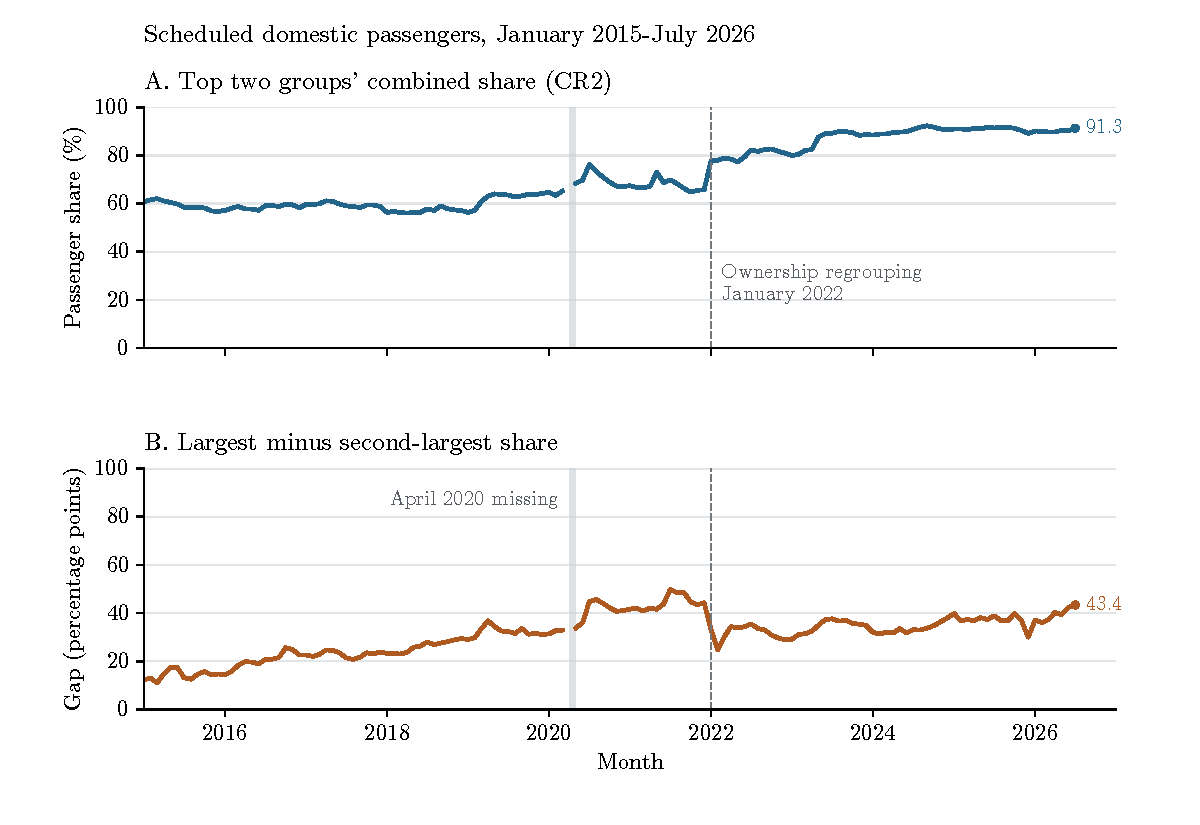
\includegraphics[width=\linewidth]{figures/o4_national_cr2_share_gap.pdf}
\caption{National concentration and share asymmetry, 2015--2026.}
\label{fig:o4-national-eda}
\vspace{2pt}
\begin{minipage}{\linewidth}
\footnotesize\setstretch{1.1}
\textit{Source:} DGCA monthly traffic via \href{https://github.com/mkubicek/india-aviation-stats/tree/16770ac59dae61ce7b80fd8bd67dd7f4cef280a6}{Kubicek (2026)}; authors' calculations.
\end{minipage}
\end{figure}

\clearpage
\subsection{O4: Route coverage and concentration}
The sample fixes the 20 busiest airport pairs by 2025 passengers, combining directions. One observation is one airport pair in one calendar month: Delhi--Mumbai in June and July count as two separate observations. There are 1,150 observations across 66 months between April 2019 and September 2026.

Panel~A of Figure~\ref{fig:o4-route-eda} counts pairs with usable data each month (12--20 in observed months). Gaps mean no retained observations, rather than zero flights.

Panel~B groups the 1,150 observations into HHI intervals of 500 points. Its horizontal axis shows HHI; its vertical axis counts observations. For example, 278 observations have HHI from 3,500 up to 4,000, so that bar has height 278. The bar heights sum to 1,150. This shows how often different concentration levels occur across the observed pairs and months, rather than how HHI changes over time.

Each observation has equal weight. Median HHI is 3,711; the middle half lies between 3,180 and 4,244. HHI uses ownership groups' approved scheduled-flight shares, not passenger shares. Appendix~\ref{app:o4-route-preparation} records preparation and exclusions.

\begin{figure}[htbp]
\centering
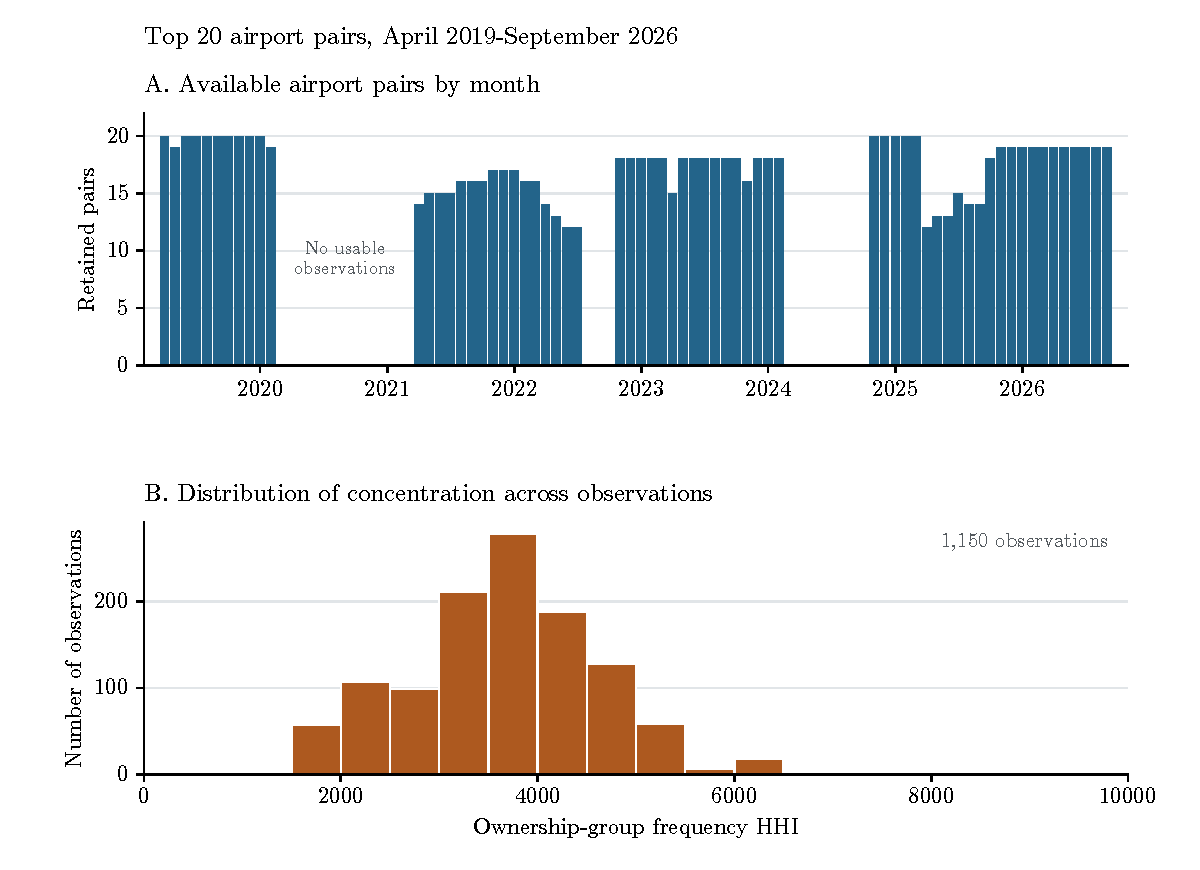
\includegraphics[width=\linewidth]{figures/o4_route_coverage_hhi.pdf}
\caption{Route-data coverage and the distribution of ownership-group frequency HHI.}
\label{fig:o4-route-eda}
\vspace{2pt}
\begin{minipage}{\linewidth}
\footnotesize\setstretch{1.1}
\textit{Source:} DGCA approved domestic schedules; authors' calculations.
\end{minipage}
\end{figure}

\clearpage
Figure~\ref{fig:o4-route-heatmap} complements the pooled histogram in Figure~\ref{fig:o4-route-eda} using the same 1,150 observations. Each row is one airport pair, ordered by 2025 passenger totals, and each column is a calendar month. Colour shows ownership-group frequency HHI on a common 0--10,000 scale; grey means no usable observation. Reading across a row shows changes for that pair, while reading down a column compares pairs in the same month. Gaps are not interpolated.

For example, Mumbai--Delhi's HHI rises from 2,071 in April 2019 to 4,146 in September 2026. The heatmap preserves this time and pair information, while the histogram shows how frequently each concentration range occurs across all observations.

\begin{figure}[htbp]
\centering
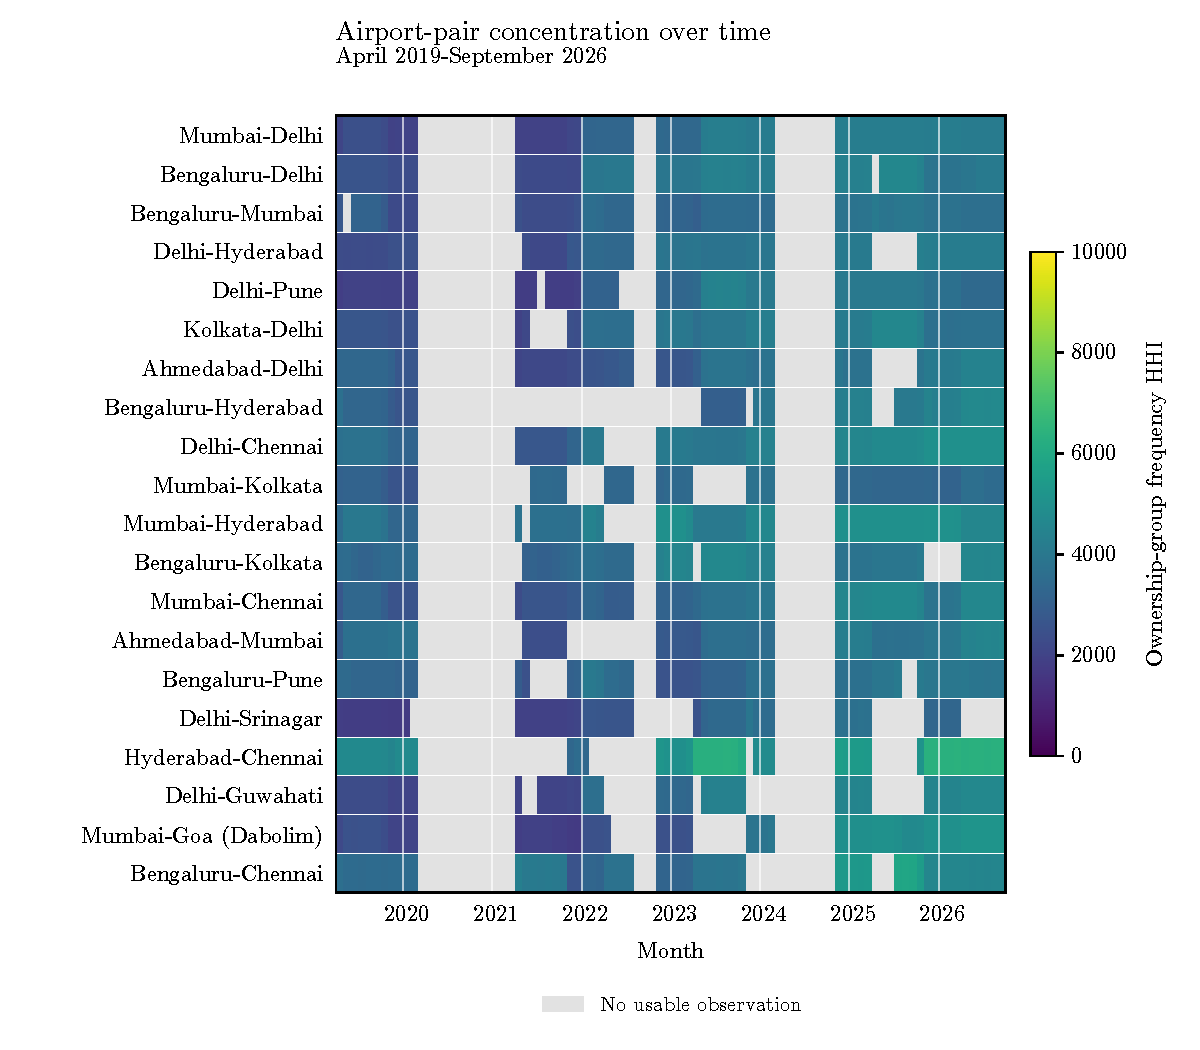
\includegraphics[width=\linewidth]{figures/o4_route_hhi_heatmap.pdf}
\caption{Ownership-group frequency HHI by airport pair and month.}
\label{fig:o4-route-heatmap}
\vspace{2pt}
\begin{minipage}{\linewidth}
\footnotesize\setstretch{1.1}
\textit{Source:} DGCA approved domestic schedules; authors' calculations.
\end{minipage}
\end{figure}

\clearpage
\subsection{O4: Capacity and passenger-traffic inputs}
Table~\ref{tab:o4-capacity-inputs} presents December 2024 and December 2025 data for scheduled domestic passenger airlines. Offered capacity, measured in available seat-kilometres (ASK), is seats offered multiplied by distance. Passenger traffic, measured in revenue passenger-kilometres (RPK), is paying passengers carried multiplied by distance. Both are reported in billions, with all airlines other than IndiGo pooled together.

IndiGo's offered capacity and passenger traffic are lower in December 2025, while both are higher for the other airlines combined. The gap between capacity and traffic supplies the input for the unused-capacity calculation in the main analysis. These national totals do not identify spare seats on a particular route or day.

\begin{minipage}{\linewidth}
\captionsetup{font=small,labelfont=bf,justification=raggedright,singlelinecheck=false,hypcap=false}
\captionof{table}{Capacity and passenger-traffic inputs for the December comparison.}
\label{tab:o4-capacity-inputs}
\centering
{\small\setstretch{1.1}\begin{tabular}{@{}llrr@{}}
\toprule
Month & Airlines & \shortstack[r]{Offered capacity\\(billion seat-km)} & \shortstack[r]{Passenger traffic\\(billion passenger-km)} \\
\midrule
Dec 2024 & IndiGo & 10.053 & 9.113 \\
Dec 2024 & Other airlines & 6.385 & 5.493 \\
Dec 2025 & IndiGo & 9.312 & 8.208 \\
Dec 2025 & Other airlines & 6.619 & 5.947 \\
\bottomrule
\end{tabular}
\par}
\vspace{4pt}
{\footnotesize\setstretch{1.1}\raggedright\textit{Source:} DGCA monthly airline traffic via \href{https://github.com/mkubicek/india-aviation-stats/tree/16770ac59dae61ce7b80fd8bd67dd7f4cef280a6}{Kubicek (2026)}; authors' calculations.\par}
\end{minipage}

\clearpage
\section{Analysis and Results}
\subsection{O4: National concentration and dominance}
IndiGo and the Air India Group are the two largest ownership groups in all 20 months from December 2024 to July 2026, with IndiGo ranked first throughout. Their combined passenger share ranges from 89.13\% to 91.70\%, and the gap between them ranges from 30.01 to 43.39 percentage points. Thus the specified pair, CR2 and gap conditions occur together in every month of this period (Table~\ref{tab:o4-national-results}).

For each month, passengers are summed within the submitted ownership groups and shares are ranked afresh. We then count months meeting each condition using unrounded values. The full-series comparison covers 138 observed months from January 2015 to July 2026; April 2020 is missing. The focus period, December 2024--July 2026, has no missing months. Appendix~\ref{app:o4-national-calculations} gives the formulas and a worked example.

\begin{minipage}{\linewidth}
\captionsetup{font=small,labelfont=bf,justification=raggedright,singlelinecheck=false,hypcap=false}
\captionof{table}{National concentration conditions: full series and December 2024--July 2026.}
\label{tab:o4-national-results}
\centering
{\small\setstretch{1.1}\setlength{\tabcolsep}{4pt}\begin{tabular}{@{}lrrr@{}}
\toprule
 & \shortstack{Full series\\Months / 138} & \shortstack{Focus period\\Months / 20} & \shortstack{Focus period\\Range} \\
\midrule
IndiGo and AI Group lead & 59/138 & 20/20 & -- \\
CR2 $\geq 80\%$ & 48/138 & 20/20 & 89.13--91.70 \\
Share gap $>20$ pp & 120/138 & 20/20 & 30.01--43.39 \\
Fringe $\leq 20\%$ & 48/138 & 20/20 & 8.30--10.87 \\
Ownership HHI $>1{,}800$ & 138/138 & 20/20 & 4,468.57--5,144.35 \\
Pair, CR2 and gap jointly & 48/138 & 20/20 & -- \\
\bottomrule
\end{tabular}
\par}
\vspace{4pt}
{\footnotesize\setstretch{1.1}\raggedright\textit{Note:} Counts give months meeting the condition / observed months. AI Group means Air India Group. CR2 and fringe are passenger percentages; the gap is in percentage points (pp); HHI is in index points. Ranges use all 20 focus-period months. The final row combines the specified pair, CR2 $\geq80\%$ and gap $>20$ pp, the conditions in H5.\par
\textit{Source:} DGCA monthly airline traffic via \href{https://github.com/mkubicek/india-aviation-stats/tree/16770ac59dae61ce7b80fd8bd67dd7f4cef280a6}{Kubicek (2026)}; authors' calculations.\par}
\end{minipage}

Across the full series, the three conditions coincide in 48 of 138 observed months (34.8\%). High HHI alone is less selective: all 138 months exceed 1,800. The measures are related: fringe is $100-\mathrm{CR2}$, and CR2 $\geq80\%$ already implies HHI $\geq3{,}200$. They are therefore not independent tests. The $>20$ pp gap is the study-defined asymmetry threshold; these descriptive cutoffs are not a legal definition of duopoly.

Under the study's ownership convention, Vistara and AirAsia India are included in the Air India Group from January 2022, having been treated separately earlier. Combining previously separate groups raises ownership HHI even if their passenger shares are unchanged. The full-series comparison therefore reflects ownership consolidation as well as changes in passenger shares.

\clearpage
\subsection{O4: Route concentration and IndiGo dependence}
\textbf{Full-period results: April 2019--September 2026.}
Ownership-group frequency HHI exceeds 1,800 in 1,143 of the 1,150 retained airport-pair/month observations (99.39\%; Table~\ref{tab:o4-route-results}). Shares are calculated from approved scheduled flights, pooling both directions before grouping airlines by ownership. Each retained observation receives equal weight. Median CR2 is 80.00\%, the median share gap is 13.73 percentage points, and median fringe share is 20.00\%.

\begin{minipage}{\linewidth}
\captionsetup{font=small,labelfont=bf,justification=raggedright,singlelinecheck=false,hypcap=false}
\captionof{table}{Route concentration and IndiGo exposure, April 2019--September 2026.}
\label{tab:o4-route-results}
\centering
{\small\setstretch{1.1}\setlength{\tabcolsep}{5pt}\begin{tabular}{@{}lrr@{}}
\toprule
Condition & Observations & Share (\%) \\
\midrule
Ownership frequency HHI $>1{,}800$ & 1,143/1,150 & 99.39 \\
Group CR2 $\geq80\%$ & 583/1,150 & 50.70 \\
Group share gap $>20$ pp & 368/1,150 & 32.00 \\
IndiGo frequency share $\geq60\%$ & 79/1,150 & 6.87 \\
IndiGo is the sole scheduled operator & 0/1,150 & 0.00 \\
IndiGo and AI Group: unique top-two pair & 730/1,150 & 63.48 \\
Unique pair, CR2 and gap conditions jointly & 95/1,150 & 8.26 \\
Tie prevents a unique top-two pair & 58/1,150 & 5.04 \\
\bottomrule
\end{tabular}
\par}
\vspace{4pt}
{\footnotesize\setstretch{1.1}\raggedright\textit{Note:} The denominator is 1,150 retained observations from 20 selected airport pairs over 66 observed months. AI Group means Air India Group. The joint row requires this unique leading pair, CR2 $\geq80\%$ and gap $>20$ pp. A tie between second and third place prevents a unique pair; exchanging first and second does not change the pair. Conditions overlap. The 60\% exposure flag is study-defined.\par
\textit{Source:} DGCA approved domestic schedules; authors' calculations.\par}
\end{minipage}

High HHI does not establish the identity of the leading groups. IndiGo and Air India Group form the unique top-two pair in 730 observations (63.48\%); 95 observations (8.26\%) also meet the CR2 and gap conditions jointly. Other unique pairs include IndiGo--Vistara (99 observations) and IndiGo--Go First (83). There are 58 observations with a tie across the second-place boundary, reported separately rather than assigned to an arbitrary pair.

IndiGo's median frequency share is 43.60\%. It supplies at least 60\% of scheduled flights in 79 observations (6.87\%), all on Bengaluru--Kolkata, Chennai--Hyderabad or Bengaluru--Chennai. Across observed months, the percentage of available sampled pairs meeting this flag ranges from 0\% to 11.11\%; none has IndiGo as the sole scheduled operator. In December 2025, one of 19 available pairs meets the flag: Chennai--Hyderabad, at 78.10\%.

HHI exceeds 1,800 in 301 of 303 exact-endpoint-match observations (99.34\%), compared with 99.39\% in the full sample. Appendix~\ref{app:o4-route-calculations} gives the workings; Appendix~\ref{app:o4-route-checks} reports the subset comparisons and leading pairs. These findings describe scheduled-frequency concentration on selected major airport pairs; they are not passenger-share estimates or network-wide measures of IndiGo dependence.

\clearpage
\subsubsection*{Matched focus period: December 2024--July 2026}
During the focus period, IndiGo and Air India Group dominate the busiest sampled airport pairs, with other airlines collectively accounting for a relatively small share. However, the gap between the two leading groups is considerably smaller than nationally: route-level dominance is shared more evenly between IndiGo and Air India.

Table~\ref{tab:o4-route-focus} compares the same 20 calendar months nationally and on the selected routes. The top 20 pairs remain the submitted sample; the top 10 form a supplementary comparison using the first ten ranks in the same fixed 2025 passenger ranking. All 20 months are represented, with 184 of 200 possible pair-months retained for the top 10 and 350 of 400 for the top 20. Unavailable pair-months are excluded.

\begin{minipage}{\linewidth}
\captionsetup{font=small,labelfont=bf,justification=raggedright,singlelinecheck=false,hypcap=false}
\captionof{table}{National and route concentration during December 2024--July 2026.}
\label{tab:o4-route-focus}
\centering
{\small\setstretch{1.1}\setlength{\tabcolsep}{4pt}\begin{tabularx}{\linewidth}{|>{\raggedright\arraybackslash}X|r|r|r|}
\hline
\textbf{Measure} & \textbf{\shortstack{\strut National\\\strut Passenger data}} & \textbf{\shortstack{\strut Top 20\\\strut airport pairs\\\strut Scheduled flights}} & \textbf{\shortstack{\strut Top 10\\\strut airport pairs\\\strut Scheduled flights}} \\
\hline
IndiGo and AI Group are the unique top two & 20/20 & 328/350 & 184/184 \\
\hline
Median CR2 (\%) & 90.91 & 89.55 & 89.37 \\
\hline
Median share gap (pp) & 37.35 & 11.92 & 7.69 \\
\hline
Median fringe share (\%) & 9.09 & 10.45 & 10.63 \\
\hline
Leading pair, CR2 $\geq80\%$ and gap $>20$ pp, with IndiGo first & 20/20 & 50/350 & 9/184 \\
\hline
\end{tabularx}
\par}
\vspace{4pt}
{\footnotesize\setstretch{1.1}\raggedright\textit{Note:} National observations are months using passenger shares; route observations are airport-pair/months using scheduled-flight-frequency shares. Each observation has equal weight within its sample. Pair counts identify the two groups regardless of which ranks first. The joint row requires that pair, CR2 $\geq80\%$, gap $>20$ pp and IndiGo ranked first. AI Group means Air India Group; pp means percentage points.\par
\textit{Source:} DGCA monthly airline traffic via Kubicek (2026) and approved domestic schedules; authors' calculations.\par}
\end{minipage}

For the top 10 pairs, IndiGo and Air India are the unique leading pair in all 184 retained observations. Their median combined share is 89.37\%, leaving a median fringe share of 10.63\%. The median gap between the two leaders is 7.69 pp, compared with 37.35 pp nationally. IndiGo ranks first in 86 observations, Air India in 94, and they tie for first in four. The unique pair, CR2 and gap conditions hold with IndiGo leading in nine observations (4.89\%).

The top 20 give a similar pattern: the two groups form the unique leading pair in 328 of 350 observations (93.71\%), with median CR2 of 89.55\% and median gap of 11.92 pp. The IndiGo-led joint conditions hold in 50 observations (14.29\%). IndiGo supplies at least 60\% of scheduled flights in 26 observations (7.43\%) in the top 20 and none in the top 10. No retained observation in either focus-period sample has IndiGo as sole operator. Appendix~\ref{app:o4-route-focus} gives the coverage and calculation details. These comparisons distinguish IndiGo's lead over Air India from the leading pair's dominance over the smaller airlines.

\clearpage
\subsection{O4: Rivals' capacity buffer}
Rivals' unused capacity relative to IndiGo's passenger traffic falls from 9.79\% in December 2024 to 8.19\% in December 2025, a decline of 1.60 percentage points (Table~\ref{tab:o4-capacity-buffer}). December 2024 provides the same-calendar-month baseline. Unused capacity is each rival's available seat-kilometres (ASK) less its revenue passenger-kilometres (RPK), summed across all retained airlines other than IndiGo. Dividing that total by IndiGo's RPK and multiplying by 100 gives the buffer measure.

\begin{minipage}{\linewidth}
\captionsetup{font=small,labelfont=bf,justification=raggedright,singlelinecheck=false,hypcap=false}
\captionof{table}{Rivals' unused capacity relative to IndiGo's traffic, December comparison.}
\label{tab:o4-capacity-buffer}
\centering
{\small\setstretch{1.1}\setlength{\tabcolsep}{5pt}\begin{tabular}{@{}lrrr@{}}
\toprule
Measure & Dec 2024 & Dec 2025 & Change \\
\midrule
Rivals' ASK (billion seat-km) & 6.385 & 6.619 & +0.234 \\
Rivals' RPK (billion passenger-km) & 5.493 & 5.947 & +0.454 \\
Rivals' unused capacity (billion seat-km) & 0.892 & 0.672 & -0.220 \\
IndiGo RPK (billion passenger-km) & 9.113 & 8.208 & -0.905 \\
Buffer relative to IndiGo (\%) & 9.79 & 8.19 & -1.60 pp \\
\bottomrule
\end{tabular}
\par}
\vspace{4pt}
{\footnotesize\setstretch{1.1}\raggedright\textit{Note:} Rivals include nine retained airline brands in December 2024 and eight in December 2025; each is counted once. Changes are December 2025 minus December 2024, calculated before rounding. The buffer denominator is IndiGo's total monthly RPK; its change is in percentage points (pp).\par
\textit{Source:} DGCA monthly airline traffic via \href{https://github.com/mkubicek/india-aviation-stats/tree/16770ac59dae61ce7b80fd8bd67dd7f4cef280a6}{Kubicek (2026)}; authors' calculations.\par}
\end{minipage}

Rivals' offered capacity rises from 6.385 to 6.619 billion seat-km, but their passenger traffic increases by more in absolute terms, from 5.493 to 5.947 billion passenger-km. The unused gap consequently narrows from 0.892 to 0.672 billion seat-km, a reduction of 24.69\%. IndiGo's RPK also falls, from 9.113 to 8.208 billion passenger-km. The buffer ratio nevertheless declines because rivals' unused capacity falls proportionately more than its denominator.

The ratios correspond to 9.79 and 8.19 unused rival seat-km per 100 IndiGo passenger-km in the respective months. They compare the aggregate buffer with all IndiGo traffic, rather than the traffic affected by cancellations. Monthly national totals do not identify whether those unused seats matched passengers' routes and travel dates, or whether airlines could add flights using available aircraft, crews and airport slots. The calculation therefore measures the size of the aggregate buffer; it does not establish actual passenger accommodation. Appendix~\ref{app:o4-capacity-buffer} gives the airline-level contributions and worked calculations.

\clearpage
\section{Discussion}
\subsection{O4: Economic interpretation}
\textbf{National asymmetry within a concentrated oligopoly.} During December 2024--July 2026, IndiGo and Air India Group carry a median 90.91\% of national passengers, leaving a median 9.09\% to the other airlines (Table~\ref{tab:o4-route-focus}). IndiGo's median lead over Air India Group is 37.35 percentage points. This pattern is consistent with an asymmetric duopoly and a small competitive fringe. Strategic interdependence is central to such a structure: capacity or pricing decisions by either large group can affect the demand faced by its rival. The shares establish the relative scale of the groups, while their actual pricing and output strategies remain unobserved.

\textbf{Market definition and route-level alternatives.} The alternatives available to a passenger depend on the journey: a seat on another airport pair does not automatically meet the same travel need. On the busiest ten sampled pairs, IndiGo and Air India are the two largest groups in all 184 retained focus-period observations. Their median combined scheduled-flight share is 89.37\%, leaving a relatively small fringe, but the median gap between the leaders is only 7.69 pp. The twenty-pair sample gives the same broad pattern. Thus the route evidence corroborates two-group dominance over the smaller airlines, while showing a more balanced division between IndiGo and Air India. National passenger shares and route scheduled-flight shares are different measures; they do not isolate the role of network coverage or establish route profitability.

\textbf{Short-run supply constraints and resilience.} Rival airlines cannot expand replacement service immediately simply because additional demand arises. Aircraft, crews and airport access constrain short-run supply, while unused seats must match passengers' routes and travel dates. The decline in rivals' unused capacity relative to IndiGo's traffic, from 9.79\% to 8.19\%, indicates less aggregate headroom in December 2025 (Table~\ref{tab:o4-capacity-buffer}). For contingency planning, the existence of another large airline therefore does not by itself establish readily available substitute capacity. The buffer describes unused seat-distance relative to IndiGo's total traffic; it measures neither actual accommodation of disrupted passengers nor short-run supply elasticity.

Concentration describes market structure, while competitive conduct and economic performance require additional evidence. A large share can reflect efficiency advantages as well as weaker competitive pressure. Without fare and cost data, these results cannot distinguish those explanations or establish effects on markups, profits or passenger welfare.

\clearpage
\subsection{O4: Hypotheses revisited}
All three O4 hypotheses are supported within their specified samples and comparison periods (Table~\ref{tab:o4-hypotheses}). These outcomes assess the descriptive conditions stated in Assignment~2; they are not statistical significance tests or causal estimates.

\begin{minipage}{\linewidth}
\captionsetup{font=small,labelfont=bf,justification=raggedright,singlelinecheck=false,hypcap=false}
\captionof{table}{O4 hypotheses: outcomes and supporting evidence.}
\label{tab:o4-hypotheses}
\centering
{\small\setstretch{1.1}\setlength{\tabcolsep}{5pt}\begin{tabular}{@{}>{\raggedright\arraybackslash}p{0.35\linewidth}>{\raggedright\arraybackslash}p{0.15\linewidth}>{\raggedright\arraybackslash}p{0.43\linewidth}@{}}
\toprule
Hypothesis & Outcome & Evidence \\
\midrule
\textbf{H5: National.} IndiGo and AI Group are the top two in every month, Dec 2024--Jul 2026, with CR2 $\geq80\%$ and gap $>20$ pp. & Supported & 20/20 months; minimum CR2 89.13\%; minimum gap 30.01 pp. Table~\ref{tab:o4-national-results}. \\
\addlinespace[6pt]
\textbf{H6: Routes.} Ownership-adjusted frequency HHI $>1{,}800$ in more than half of available observations for the selected 20 pairs. & Supported & 1,143/1,150 pair-months (99.39\%) exceed 1,800. Table~\ref{tab:o4-route-results}. \\
\addlinespace[6pt]
\textbf{H7: Buffer.} Rivals' unused capacity relative to IndiGo RPK is lower in Dec 2025 than Dec 2024. & Supported & 9.7905\% to 8.1865\%; change -1.6040 pp. Table~\ref{tab:o4-capacity-buffer}. \\
\bottomrule
\end{tabular}
\par}
\vspace{4pt}
{\footnotesize\setstretch{1.1}\raggedright\textit{Note:} AI Group means Air India Group; pp means percentage points. H6 uses the full April 2019--September 2026 route sample. The H7 denominator is IndiGo's total monthly RPK.\par
\textit{Source:} Authors' calculations from the Section~5 data.\par}
\end{minipage}

H6 concerns high route concentration, rather than requiring IndiGo to lead Air India by a large margin on every pair. The focus-period comparison therefore qualifies the broader description of asymmetry without contradicting H6: the two groups dominate the busiest sampled pairs, but their scheduled-flight shares are more evenly balanced than their national passenger shares. H7 supports a smaller aggregate buffer, without establishing how many disrupted passengers could actually be accommodated.

\textcite{kumari2026soaring} find that operational efficiency, particularly passenger load factor, matters for airline profitability alongside market structure. Our results preserve that distinction: H5 and H6 establish concentration under the specified measures, while the capacity comparison adds evidence about unused seat-distance. The route results extend the national perspective by distinguishing dominance over the fringe from the gap between the two leaders; they do not replicate the paper's profitability tests or establish collusion.

\textcite{gupta2025antitrust} warn that dependence on a dominant airline can magnify disruption risks. Our capacity comparison adds descriptive evidence of a declining buffer, without establishing that concentration caused the disruption or prevented recovery.

\section{Implications and Recommendations}
Discuss the implications of the findings for the relevant stakeholders.

Depending on the topic, these may include:
\templatebullet{Firms and managers}
\templatebullet{Consumers}
\templatebullet{Regulators}
\templatebullet{Policymakers}
\templatebullet{Industry participants}
Provide 2--3 specific recommendations where appropriate. Recommendations should follow from the findings of the study.

\clearpage
\section{Limitations}
\subsection{O4: Measurement, coverage and interpretation}
\textbf{Scheduled frequency versus passengers carried.} Route concentration uses approved scheduled-flight frequencies, while national concentration uses passenger shares. Flights differ in aircraft size and occupancy, and schedules may differ from actual operations. Consequently, the smaller IndiGo--Air India gap on busy airport pairs describes scheduled frequency; it does not establish an equally balanced division of route passengers. The findings also cannot determine how much of the national--route difference comes from network coverage, aircraft size or occupancy. Airline-by-route passenger and operated-flight data would allow a closer comparison.

\textbf{Incomplete coverage and selected airport pairs.} The sample fixes the twenty busiest pairs by 2025 passengers. In the matched focus period, 350 of 400 possible top-20 pair-months are available; the top-ten comparison retains 184 of 200. These observations need not represent missing pair-months or smaller routes elsewhere in the network. Source-quality screens and the two documented TruJet-related exclusions improve consistency but cannot detect every missing airline filing. Although 99.34\% of exact-endpoint-match observations exceed HHI 1,800, compared with 99.39\% overall, this does not establish complete coverage or random missingness.

\textbf{Aggregate capacity buffer.} The fall from 9.79\% to 8.19\% compares monthly unused rival seat-kilometres with all IndiGo passenger-kilometres, rather than the traffic affected by cancellations. It does not show whether unused seats were available on the required routes and dates, or whether additional aircraft, crews and airport slots could be deployed. The two-December comparison is descriptive and cannot establish the cause of the smaller buffer or actual passenger accommodation. Assessing recovery would require disruption-specific demand and route/date-specific available capacity.

\textbf{Ownership conventions and limits to inference.} The January 2022 ownership regrouping mechanically changes concentration, so movements around that date cannot be attributed entirely to passenger redistribution. April 2020 is missing nationally and is not imputed; pandemic-era changes also complicate comparisons across the full series. The gap and IndiGo-exposure thresholds are study-defined descriptive flags. The observed persistence of the national pattern does not establish that it will continue beyond July 2026. Without fare, marginal-cost and recovery data, concentration and buffer measures cannot establish collusion, fare effects, profitability or passenger harm.

\section{Conclusion}
Summarise the research question, main findings, key economic interpretation, and main implications.

\newpage
\nocite{kubicek2026aviationstats,dgcaDomesticSchedules}
\printbibliography[title={References}]

\newpage
\appendix
\section{Variable Dictionary}
\label{app:o4-dictionary}
\subsection{O4: Observation keys and inputs}
The dictionary covers the inputs, measures and flags used in O4's reported analysis and supporting outputs. National observations are market-months; route observations are airport-pair/months. Detailed extraction-column and CSV documentation accompanies the code repository.

\begin{minipage}{\linewidth}
\captionsetup{font=small,labelfont=bf,justification=raggedright,singlelinecheck=false,hypcap=false}
\captionof{table}{O4 observation keys and input variables.}
\label{tab:o4-dictionary-inputs}
\centering
{\footnotesize\setstretch{1.0}\setlength{\tabcolsep}{4pt}\begin{tabular}{@{}>{\raggedright\arraybackslash}p{0.24\linewidth}>{\raggedright\arraybackslash}p{0.59\linewidth}>{\raggedright\arraybackslash}p{0.12\linewidth}@{}}
\toprule
Variable / key & Meaning and construction & Unit \\
\midrule
Month & Calendar month. National and capacity CSVs use a first-of-month date (YYYY-MM-01); route CSVs use YYYY-MM. & Month \\
\addlinespace[5pt]
Airline brand & Standardised operating-brand label. Positive-passenger scheduled-domestic records form the national and capacity samples. & Category \\
\addlinespace[5pt]
Ownership group & Airline brands combined under the study's common-ownership convention; group passengers or flights are summed before shares are calculated. & Category \\
\addlinespace[5pt]
Airport pair & Unordered pair of airport codes, with both directions pooled. A pair in one month is one route observation. GOI and GOX remain separate airports. & Identifier \\
\addlinespace[5pt]
2025 route passengers and rank & Passenger journeys summed over both directions and all twelve months of 2025. Descending totals fix the top-twenty selection and its top-ten subset for every study month. These data have no airline breakdown. & Journeys; rank \\
\addlinespace[5pt]
National passengers, $P_{gt}$ & Passenger journeys carried by ownership group $g$ in month $t$, summed over retained airline brands. These are journeys, not unique travellers. & Journeys \\
\addlinespace[5pt]
Scheduled flights, $f_{grt}$ & Approved scheduled departures for group $g$, pair $r$, month $t$, pooling both directions. Weekdays and validity dates are expanded; each airline/flight/date/directed-leg event is counted once. & Flights \\
\addlinespace[5pt]
ASK and RPK & ASK is seats offered times distance; RPK is revenue passengers carried times distance. Reported source values are in thousands; dividing by 1,000,000 expresses them in billions. & Seat-km; passenger-km \\
\bottomrule
\end{tabular}
\par}
\vspace{4pt}
{\footnotesize\setstretch{1.0}\raggedright\textit{Source:} Authors' definitions based on the DGCA inputs used in O4.\par}
\end{minipage}

\textbf{Ownership convention.} Air India and Air India Express are combined throughout, as are Jet Airways and JetLite. Vistara and AirAsia India/AIX Connect also join Air India Group from January 2022; they are separate earlier. Other brands, including Alliance Air, remain separate.

\textbf{Periods and sample flags.} National: January 2015--July 2026, excluding missing April 2020. Routes: available April 2019--September 2026. Focus period: December 2024--July 2026. Top-ten membership selects fixed ranks 1--10. The buffer compares December 2024 with December 2025.

\clearpage
\subsection{O4: Constructed measures}
In Table~\ref{tab:o4-dictionary-measures}, $g$ denotes an ownership group, $r$ an airport pair and $t$ a month. Shares $s$ are percentages, and subscripts $(1)$ and $(2)$ identify the largest and second-largest shares in the observation. Percentage points are abbreviated pp.

\begin{minipage}{\linewidth}
\captionsetup{font=small,labelfont=bf,justification=raggedright,singlelinecheck=false,hypcap=false}
\captionof{table}{O4 constructed measures and units.}
\label{tab:o4-dictionary-measures}
\centering
{\footnotesize\setstretch{1.0}\setlength{\tabcolsep}{4pt}\begin{tabular}{@{}>{\raggedright\arraybackslash}p{0.24\linewidth}>{\raggedright\arraybackslash}p{0.59\linewidth}>{\raggedright\arraybackslash}p{0.12\linewidth}@{}}
\toprule
Measure & Definition & Unit \\
\midrule
National group share & $s_{gt}=100P_{gt}/\sum_gP_{gt}$, using monthly passenger journeys. & \% \\
\addlinespace[5pt]
Route group share & $s_{grt}=100f_{grt}/\sum_gf_{grt}$, using scheduled flights on the pair in that month. & \% \\
\addlinespace[5pt]
Ownership / brand HHI & $\sum s^2$, with shares on the 0--100 scale. Ownership HHI sums squared group shares; brand HHI instead treats each operating brand separately. & Index points \\
\addlinespace[5pt]
CR2 & $s_{(1)}+s_{(2)}$, the combined share of the two largest groups, ranked afresh for each observation. & \% \\
\addlinespace[5pt]
Leader--rival gap & $s_{(1)}-s_{(2)}$. Nonnegative; this compares the two largest groups, whichever group leads. & pp \\
\addlinespace[5pt]
Fringe share & $100-\mathrm{CR2}$. Combined share of all groups outside the leading pair. & \% \\
\addlinespace[5pt]
IndiGo / AI frequency share & Each named group's scheduled flights divided by all scheduled flights on the pair in that month, times 100. & \% \\
\addlinespace[5pt]
Signed IndiGo--AI gap & IndiGo's frequency share minus Air India Group's. Unlike the leader--rival gap, it can be negative; retained in the focus-period CSV. & pp \\
\addlinespace[5pt]
Unused rival capacity, $U_t$ & $\sum_{j\ne I}(\mathrm{ASK}_{jt}-\mathrm{RPK}_{jt})$, where $I$ is IndiGo. Every retained rival brand is counted once. & Seat-km \\
\addlinespace[5pt]
Buffer relative to IndiGo, $B_t$ & $100U_t/\mathrm{RPK}_{It}$. The denominator is all IndiGo monthly RPK, not rivals' ASK or cancellation-affected traffic. & \% \\
\addlinespace[5pt]
Buffer change / unused-capacity change & $B_{2025}-B_{2024}$ is the buffer change in pp. $100(U_{2025}/U_{2024}-1)$ is the percentage change in unused capacity, comparing the two Decembers. & pp; \% \\
\addlinespace[5pt]
Exposure / condition percentages & Monthly exposure: 100 times flagged pairs divided by retained pairs that month. Pooled percentages: 100 times qualifying pair-months divided by all retained pair-months in the stated sample. & \% \\
\addlinespace[5pt]
Summary statistics & Means, medians, sample standard deviations and ranges use equally weighted observations within the stated sample. Route quartiles use linear interpolation. & Measure's unit \\
\bottomrule
\end{tabular}
\par}
\vspace{4pt}
{\footnotesize\setstretch{1.0}\raggedright\textit{Source:} Definitions implemented in the O4 analysis code.\par}
\end{minipage}

All calculations precede display rounding. Pooled route summaries weight pair-months equally; pairs with more retained months contribute more observations. HHI ranges from zero to 10,000 in principle. Source and display capacity units differ only in scale; missing values are not zero.

\clearpage
\subsection{O4: Flags, coverage and missingness}
Boolean flags are saved as True/False. Table~\ref{tab:o4-dictionary-flags} defines the conditions behind the reported counts. These descriptive flags do not identify pricing conduct or constitute independent tests of duopoly.

\begin{minipage}{\linewidth}
\captionsetup{font=small,labelfont=bf,justification=raggedright,singlelinecheck=false,hypcap=false}
\captionof{table}{O4 analytical flags and source-quality conventions.}
\label{tab:o4-dictionary-flags}
\centering
{\footnotesize\setstretch{1.0}\setlength{\tabcolsep}{4pt}\begin{tabular}{@{}>{\raggedright\arraybackslash}p{0.24\linewidth}>{\raggedright\arraybackslash}p{0.59\linewidth}>{\raggedright\arraybackslash}p{0.12\linewidth}@{}}
\toprule
Flag / convention & Rule and interpretation & Unit \\
\midrule
Concentration flags & True when ownership HHI $>1{,}800$, CR2 $\geq80\%$, gap $>20$ pp or fringe $\leq20\%$, respectively. CR2 and fringe conditions are equivalent; gap $>20$ pp is study-defined. & Boolean \\
\addlinespace[5pt]
IndiGo exposure / sole operator & Exposure is True when IndiGo supplies $\geq60\%$ of scheduled flights (study-defined). Sole operator is True only when all scheduled flights belong to IndiGo. & Boolean \\
\addlinespace[5pt]
Leading-group identities and ties & Groups rank by passengers nationally or flights on each pair-month. Alphabetical ordering resolves ties for display. A route tie across ranks two and three prevents a unique top-two pair; a two-way first-place tie alone does not. & Categories; Boolean \\
\addlinespace[5pt]
IndiGo--AI leading-pair flag & True when the top two are IndiGo and Air India Group, regardless of order. The route ``unique pair'' flag also requires no tie across ranks two and three. & Boolean \\
\addlinespace[5pt]
Joint concentration flags & H5 combines the national pair flag with CR2 $\geq80\%$ and gap $>20$ pp. The route joint flag applies those conditions to the unique pair; the IndiGo-led variant additionally requires IndiGo to lead. H6 counts observations using only the HHI flag. & Boolean \\
\addlinespace[5pt]
First-place leadership flags & IndiGo or AI is a unique leader only if its share strictly exceeds every rival's. First-place ties are counted separately, including in focus-period leadership totals. & Boolean \\
\addlinespace[5pt]
Endpoint discrepancy / exact match & Discrepancy is 100 times the sum of absolute airline departure--arrival count differences divided by total departures, pooling directions. Exact match is True only if each airline's two totals agree. & \%; Boolean \\
\addlinespace[5pt]
Retained pair-month / available pairs & Retention requires full-month source coverage, endpoint discrepancy $\leq5\%$ and at least ten qualifying pairs in the full twenty-pair panel that month, after exclusions. HYD--MAA in February--March 2022 is excluded. Available pairs count retained observations in the month. & Boolean; count \\
\addlinespace[5pt]
Capacity validity & A valid positive-passenger record has ASK $>0$ and $0\leq\mathrm{RPK}\leq\mathrm{ASK}$. Invalid records remain flagged without imputation; the buffer calculation requires every selected December record to be valid. & Category \\
\bottomrule
\end{tabular}
\par}
\vspace{4pt}
{\footnotesize\setstretch{1.0}\raggedright\textit{Source:} Rules implemented in the O4 preparation and analysis code.\par}
\end{minipage}

\textbf{Missingness.} Unavailable or excluded pair-months are absent from analysis tables and blank in the heatmap matrix (grey in the figure). Zero available pairs means no retained data, not zero flights. Coverage checks do not prove all filings are present. Observed zero gaps, fringe shares or exposure counts remain valid values. Preparation and workings are in Appendix~\ref{app:o4-route-preparation}.

\clearpage
\section{Additional Tables and Figures}
\label{app:o4-national-summary}
\begin{minipage}{\linewidth}
\captionsetup{font=small,labelfont=bf,justification=raggedright,singlelinecheck=false,hypcap=false}
\captionof{table}{National concentration: descriptive statistics, January 2015--July 2026.}
\label{tab:o4-national-summary}
\centering
{\small\setstretch{1.1}\begin{tabular}{@{}lrrrrr@{}}
\toprule
Measure & Mean & Median & Std. dev. & Minimum & Maximum \\
\midrule
Ownership HHI (points) & 3,446.95 & 3,367.72 & 991.68 & 2,216.18 & 5,144.35 \\
CR2 (\%) & 71.97 & 66.90 & 13.43 & 56.09 & 92.30 \\
Share gap (pp) & 30.92 & 32.24 & 8.87 & 11.11 & 49.87 \\
Fringe share (\%) & 28.03 & 33.10 & 13.43 & 7.70 & 43.91 \\
\bottomrule
\end{tabular}
\par}
\vspace{4pt}
{\footnotesize\setstretch{1.1}\raggedright\textit{Note:} Each measure has 138 observed months, weighted equally. April 2020 is missing and is not imputed. HHI uses squared ownership-group percentage shares; CR2 adds the largest two shares, the gap subtracts the second from the first, and fringe share is $100-\mathrm{CR2}$. Standard deviations use the sample formula; pp means percentage points.\par
\textit{Source:} DGCA monthly airline traffic via Kubicek (2026); authors' calculations.\par}
\end{minipage}

\clearpage
\section{Additional Analysis}
\label{app:o4-route-preparation}
\subsection{O4: National concentration calculations}
\label{app:o4-national-calculations}
For ownership group $g$ in month $t$, let $q_{gt}$ be passengers and $Q_t=\sum_g q_{gt}$. Its percentage share is $s_{gt}=100q_{gt}/Q_t$. Rank shares each month as $s_{1t}\geq s_{2t}\geq\cdots$. Calculate
\[
\begin{aligned}
\mathrm{CR2}_t&=s_{1t}+s_{2t}, &\quad \mathrm{Gap}_t&=s_{1t}-s_{2t},\\
\mathrm{Fringe}_t&=100-\mathrm{CR2}_t, &\quad \mathrm{HHI}_t&=\sum_g s_{gt}^{2}.
\end{aligned}
\]
The joint count includes a month only when the top-two groups are IndiGo and Air India Group, CR2 $\geq80\%$ and gap $>20$ pp. Divide this count by observed months to obtain the percentage. Missing months are excluded, not assigned zero. CR2 $\geq80\%$ implies $s_1^2+s_2^2\geq(s_1+s_2)^2/2\geq3{,}200$, before adding the other groups' contributions.

\begin{minipage}{\linewidth}
\captionsetup{font=small,labelfont=bf,justification=raggedright,singlelinecheck=false,hypcap=false}
\captionof{table}{Worked national concentration inputs and HHI contributions, July 2026.}
\label{tab:o4-national-worked}
\centering
{\small\setstretch{1.1}\begin{tabular}{@{}lrrr@{}}
\toprule
Ownership group & Passengers & Share (\%) & HHI contribution \\
\midrule
IndiGo & 8,081,825 & 67.3518 & 4,536.27 \\
Air India Group & 2,875,100 & 23.9603 & 574.10 \\
Akasa Air & 664,572 & 5.5384 & 30.67 \\
SpiceJet & 187,280 & 1.5607 & 2.44 \\
Star Air & 83,018 & 0.6919 & 0.48 \\
Fly91 & 56,152 & 0.4680 & 0.22 \\
Alliance Air & 50,078 & 0.4173 & 0.17 \\
India One Air & 1,386 & 0.0116 & 0.00 \\
\midrule
Total & 11,999,411 & 100.0000 & 5,144.35 \\
\bottomrule
\end{tabular}
\par}
\vspace{4pt}
{\footnotesize\setstretch{1.1}\raggedright\textit{Note:} Each HHI contribution is the square of its group's percentage share. Calculations use unrounded shares; displayed shares and contributions are rounded independently.\par
\textit{Source:} Same passenger snapshot and ownership convention as Table~\ref{tab:o4-national-results}; authors' calculations.\par}
\end{minipage}

For example, IndiGo's share is $100\times8{,}081{,}825/11{,}999{,}411\approx67.3518\%$. Using all groups in Table~\ref{tab:o4-national-worked} gives
\begin{align*}
\mathrm{CR2} &\approx 67.3518+23.9603 \approx 91.3122\%, \\
\mathrm{Gap} &\approx 67.3518-23.9603 \approx 43.3915\ \mathrm{pp}, \\
\mathrm{Fringe} &\approx 100-91.3122 \approx 8.6878\%, \\
\mathrm{HHI} &= \sum_g s_g^2 \approx 5,144.35.
\end{align*}

July 2026 meets all three joint conditions and contributes one month to the numerator. Repeating this calculation gives $48/138\times100\approx34.8\%$ for the full series and $20/20\times100=100\%$ for December 2024--July 2026.

\clearpage
\subsection{O4: Route concentration calculations}
\label{app:o4-route-calculations}
For group $g$ on airport pair $r$ in month $t$, let $f_{grt}$ be scheduled flights after pooling both directions and $F_{rt}=\sum_g f_{grt}$. Percentage shares are $s_{grt}=100f_{grt}/F_{rt}$; CR2, gap, fringe and HHI follow the formulas in Appendix~\ref{app:o4-national-calculations}. The shares here measure scheduled frequency rather than national passengers.

The numerator for H6 counts retained observations with HHI $>1{,}800$; the denominator is all 1,150 retained observations. Thus $1{,}143/1{,}150\times100\approx99.39\%$. The corresponding IndiGo exposure calculation is $79/1{,}150\times100\approx6.87\%$, using its $\geq60\%$ frequency-share flag. These are pooled observation percentages. Monthly route percentages instead divide the number meeting a condition by the number of available pairs in that month, which is not always 20.

\begin{minipage}{\linewidth}
\captionsetup{font=small,labelfont=bf,justification=raggedright,singlelinecheck=false,hypcap=false}
\captionof{table}{Worked route concentration inputs: Delhi--Pune, June 2026.}
\label{tab:o4-route-worked}
\centering
{\small\setstretch{1.1}\begin{tabular}{@{}lrrr@{}}
\toprule
Group & Scheduled flights & Share (\%) & HHI contribution \\
\midrule
Air India Group & 618 & 43.2168 & 1,867.69 \\
IndiGo & 524 & 36.6434 & 1,342.74 \\
SpiceJet & 168 & 11.7483 & 138.02 \\
Akasa Air & 120 & 8.3916 & 70.42 \\
\midrule
Total & 1,430 & 100.0000 & 3,418.87 \\
\bottomrule
\end{tabular}
\par}
\vspace{4pt}
{\footnotesize\setstretch{1.1}\raggedright\textit{Note:} The 618 Air India Group flights combine Air India (472) and Air India Express (146). HHI contributions square group percentage shares. Calculations use unrounded shares; displayed components are rounded independently.\par
\textit{Source:} Prepared DGCA approved schedules; authors' calculations.\par}
\end{minipage}

The Air India Group has the largest frequency share and IndiGo the second largest:
\begin{align*}
\mathrm{CR2} &\approx 43.2168+36.6434 \approx 79.8601\%, \\
\mathrm{Gap} &\approx 43.2168-36.6434 \approx 6.5734\ \mathrm{pp}, \\
\mathrm{Fringe} &\approx 100-79.8601 \approx 20.1399\%, \\
\mathrm{HHI} &= \sum_g s_g^2 \approx 3,418.87, \\
s_{\mathrm{IndiGo}} &= 100\times524/1430 \approx 36.6434\%.
\end{align*}

This observation contributes to the HHI-above-1,800 count and the unique IndiGo--Air India leading-pair count. It does not meet CR2 $\geq80\%$, gap $>20$ pp or IndiGo share $\geq60\%$. The same steps are repeated separately for each retained pair and month.

\clearpage
\subsection{O4: Route subset comparisons and leading pairs}
\label{app:o4-route-checks}
Table~\ref{tab:o4-route-sensitivity} compares the full sample with the stricter exact-endpoint-match subset. December 2025 is a separate period comparison. Exact matches refer to airline arrival and departure counts agreeing, not proof that every airline filing is present. The subsets overlap and should not be added together.

\begin{minipage}{\linewidth}
\captionsetup{font=small,labelfont=bf,justification=raggedright,singlelinecheck=false,hypcap=false}
\captionof{table}{Route concentration and IndiGo exposure across sample definitions.}
\label{tab:o4-route-sensitivity}
\centering
{\small\setstretch{1.1}\setlength{\tabcolsep}{4pt}\begin{tabular}{@{}lrrr@{}}
\toprule
Sample & $N$ & HHI $>1{,}800$: $n$ (\%) & IndiGo $\geq60\%$: $n$ (\%) \\
\midrule
Full sample & 1,150 & 1,143 (99.39\%) & 79 (6.87\%) \\
Exact endpoint matches & 303 & 301 (99.34\%) & 26 (8.58\%) \\
December 2025 & 19 & 19 (100.00\%) & 1 (5.26\%) \\
\bottomrule
\end{tabular}
\par}
\vspace{4pt}
{\footnotesize\setstretch{1.1}\raggedright\textit{Note:} $N$ is retained airport-pair/month observations and $n$ is observations meeting each condition. Exact matches and December 2025 are subsets of April 2019--September 2026. No subset contains an IndiGo-only observation.\par
\textit{Source:} DGCA approved domestic schedules; authors' calculations.\par}
\end{minipage}

\begin{minipage}{\linewidth}
\captionsetup{font=small,labelfont=bf,justification=raggedright,singlelinecheck=false,hypcap=false}
\captionof{table}{Leading ownership-group pairs across the 1,150 retained observations.}
\label{tab:o4-route-leaders}
\centering
{\small\setstretch{1.1}\setlength{\tabcolsep}{4pt}\begin{tabular}{@{}lrr@{}}
\toprule
Top-two ownership groups & Observations & Share (\%) \\
\midrule
Air India Group + IndiGo & 730 & 63.48 \\
IndiGo + Vistara & 99 & 8.61 \\
Go First / GoAir + IndiGo & 83 & 7.22 \\
IndiGo + SpiceJet & 78 & 6.78 \\
Tie at second place & 58 & 5.04 \\
AirAsia India / AIX Connect + IndiGo & 50 & 4.35 \\
Akasa Air + IndiGo & 23 & 2.00 \\
Air India Group + Go First / GoAir & 13 & 1.13 \\
Alliance Air + IndiGo & 8 & 0.70 \\
Go First / GoAir + SpiceJet & 6 & 0.52 \\
Air India Group + Vistara & 1 & 0.09 \\
Go First / GoAir + Vistara & 1 & 0.09 \\
\bottomrule
\end{tabular}
\par}
\vspace{4pt}
{\footnotesize\setstretch{1.1}\raggedright\textit{Note:} Pair order does not indicate which group ranks first. When ranks two and three have equal flight counts, the observation is assigned to the tie category. This changes pair identification, not HHI, CR2, gap or fringe. Counts sum to 1,150.\par
\textit{Source:} DGCA approved domestic schedules; authors' calculations.\par}
\end{minipage}

\clearpage
\subsection{O4: Matched focus-period calculations and coverage}
\label{app:o4-route-focus}
The focus-period comparison retains observations dated December 2024--July 2026. The top-10 subset uses ranks 1--10 in the fixed 2025 passenger ranking; the submitted top-20 sample is unchanged. Table~\ref{tab:o4-focus-coverage} gives each month's available pairs. Missing observations are excluded, giving 184 retained pair-months for the top 10 and 350 for the top 20. Every calendar month is represented in both samples.

\begin{minipage}{\linewidth}
\captionsetup{font=small,labelfont=bf,justification=raggedright,singlelinecheck=false,hypcap=false}
\captionof{table}{Retained airport pairs in each focus-period month.}
\label{tab:o4-focus-coverage}
\centering
{\small\setstretch{1.1}\begin{tabular}{@{}lrr@{}}
\toprule
Month & Top 10 retained & Top 20 retained \\
\midrule
2024-12 & 10/10 & 20/20 \\
2025-01 & 10/10 & 20/20 \\
2025-02 & 10/10 & 20/20 \\
2025-03 & 10/10 & 20/20 \\
2025-04 & 6/10 & 12/20 \\
2025-05 & 7/10 & 13/20 \\
2025-06 & 7/10 & 13/20 \\
2025-07 & 8/10 & 15/20 \\
2025-08 & 8/10 & 14/20 \\
2025-09 & 8/10 & 14/20 \\
2025-10 & 10/10 & 18/20 \\
2025-11 & 10/10 & 19/20 \\
2025-12 & 10/10 & 19/20 \\
2026-01 & 10/10 & 19/20 \\
2026-02 & 10/10 & 19/20 \\
2026-03 & 10/10 & 19/20 \\
2026-04 & 10/10 & 19/20 \\
2026-05 & 10/10 & 19/20 \\
2026-06 & 10/10 & 19/20 \\
2026-07 & 10/10 & 19/20 \\
\midrule
Total pair-months & 184/200 & 350/400 \\
\bottomrule
\end{tabular}
\par}
\vspace{4pt}
{\footnotesize\setstretch{1.1}\raggedright\textit{Source:} Prepared DGCA approved schedules and source-quality screen; authors' calculations.\par}
\end{minipage}

Shares and indices are calculated separately for each retained pair-month using Appendix~\ref{app:o4-route-calculations}. Reported medians are taken across these observations with equal weight; they are not averages of monthly medians or pooled flight shares. The IndiGo-led joint count requires the unique IndiGo--Air India pair, CR2 $\geq80\%$, gap $>20$ pp and IndiGo ranked first:
\begin{align*}
\text{Top 10, IndiGo-led joint share} &= 100\times9/184 \approx 4.89\%, \\
\text{Top 20, IndiGo-led joint share} &= 100\times50/350 \approx 14.29\%.
\end{align*}

First-place ties are counted separately: IndiGo leads in 86, Air India in 94 and both tie in four top-10 observations; the corresponding top-20 counts are 214, 132 and four.

\clearpage
\subsection{O4: Capacity-buffer calculations}
\label{app:o4-capacity-buffer}
Let $I$ denote IndiGo and $j$ a retained rival airline brand. For month $t$, unused rival capacity $U_t$ and the buffer percentage $B_t$ are
\[
U_t=\sum_{j\ne I}(\mathrm{ASK}_{jt}-\mathrm{RPK}_{jt}),
\qquad B_t=100\frac{U_t}{\mathrm{RPK}_{It}}.
\]
The same positive-passenger scheduled-domestic filter is used as in Section~4.3. All 19 selected airline records have valid ASK/RPK inputs. The source reports thousands of seat-km and passenger-km; dividing by 1,000,000 expresses them in billions. Summing the airline-level unused amounts gives the numerator in Table~\ref{tab:o4-capacity-buffer}.

\begin{minipage}{\linewidth}
\captionsetup{font=small,labelfont=bf,justification=raggedright,singlelinecheck=false,hypcap=false}
\captionof{table}{Rival contributions to unused capacity, billion seat-kilometres.}
\label{tab:o4-capacity-buffer-airlines}
\centering
{\small\setstretch{1.1}\begin{tabular}{@{}lrr@{}}
\toprule
Rival airline & Dec 2024 & Dec 2025 \\
\midrule
Air India & 0.536252 & 0.285438 \\
Air India Express & 0.202121 & 0.229222 \\
Akasa Air & 0.058291 & 0.042310 \\
Alliance Air & 0.011655 & 0.010020 \\
Fly91 & 0.002312 & 0.002727 \\
Flybig & 0.001020 & -- \\
India One Air & 0.000148 & 0.000193 \\
SpiceJet & 0.071044 & 0.087059 \\
Star Air & 0.009372 & 0.014969 \\
\midrule
Total & 0.892215 & 0.671937 \\
\bottomrule
\end{tabular}
\par}
\vspace{4pt}
{\footnotesize\setstretch{1.1}\raggedright\textit{Note:} Each value is that airline's ASK minus RPK. A dash denotes no retained positive-passenger record, not an imputed zero. Totals and individual values are rounded independently. IndiGo is excluded from these sums and supplies only the ratio's RPK denominator.\par
\textit{Source:} DGCA monthly airline traffic via Kubicek (2026); authors' calculations.\par}
\end{minipage}

Using billions for both numerator and denominator gives
\begin{align*}
U_{2024} &= 6.384761131-5.492545663=0.892215468, \\
U_{2025} &= 6.618678370-5.946741054=0.671937316, \\
B_{2024} &=100\times\frac{0.892215468}{9.113052}\approx 9.7905\%, \\
B_{2025} &=100\times\frac{0.671937316}{8.207875}\approx 8.1865\%, \\
\Delta B &= B_{2025}-B_{2024}\approx -1.6040\ \mathrm{pp}, \\
\text{Change in unused capacity} &=100\left(\frac{U_{2025}}{U_{2024}}-1\right)\approx -24.69\%.
\end{align*}

The denominator is all IndiGo RPK in each December. The CSV outputs preserve every airline's ASK/RPK inputs and the unrounded aggregates, ratios and change.

\clearpage
\subsection{O4: Reproduction and data preparation}

\textbf{O4 reproduction files.} Data preparation, Python plotting code, numerical tables and run instructions are available in the \href{https://github.com/Goutham7358/Assignment3_Code}{Assignment 3 code repository}.

\textbf{O4 capacity preparation.} Capacity records use the same positive-passenger scheduled-domestic filter as the national passenger panel. Source ASK and RPK are in thousands; the table divides by 1,000,000 to express them in billions. Both December samples have valid positive capacity and traffic values (ten airline brands in 2024, nine in 2025). Two earlier positive-passenger records, Air Odisha in September 2018 and Air Deccan in March 2020, report zero ASK and RPK. They remain flagged in the prepared capacity CSV and are not imputed; neither enters the December comparison.

\textbf{O4 route preparation.} The archive contains 228 DGCA schedule PDFs; 92 contribute departure rows to the retained sample. Extraction preserves PDF, page and row references. Flight weekdays and validity dates are expanded into calendar dates, duplicate flight-date-directed legs are removed, and directions are pooled before shares are calculated. The top 20 pairs are selected using 2025 passenger totals from the \href{https://github.com/mkubicek/india-aviation-stats/tree/16770ac59dae61ce7b80fd8bd67dd7f4cef280a6}{DGCA-derived dataset distributed by Kubicek (2026)}.

The source-quality screen requires full-month source coverage, a sum of absolute airline endpoint-count differences no greater than 5\% of departures, and at least ten retained pairs per month. Chennai--Hyderabad in February and March 2022 is excluded because the archived TruJet plan extends beyond its suspension. This removes two observations from the earlier 1,152-observation panel, consistently with the O3 treatment. Of the 1,150 retained observations, 303 have exactly matching endpoint counts. Missing carrier filings can escape these checks; the series describes recovered approved schedules, not actual operations or airline passenger shares.

\section{Survey Questionnaire or Interview Guide}
Include the survey questionnaire or interview guide where applicable.

\newpage
\section*{Methods and Tools Statement}
Provide a short statement covering:
\templatebullet{Data sources used}
\templatebullet{Software or analytical tools used}
\templatebullet{Other relevant tools used in preparing or analysing the study}
\templatebullet{Any AI tool assistance, where applicable}

\section*{Team Member Contributions}
Provide one line for each team member describing their contribution to the project.

This statement is intended only to confirm that all team members have contributed to the project. It is not an individual assessment of the quality or quantity of each member's contribution, and differences in individual contributions will not result in different marks for team members.
\templatebullet{\textbf{[Member 1]:} [Brief description of contribution.]}
\templatebullet{\textbf{[Member 2]:} [Brief description of contribution.]}
\templatebullet{\textbf{[Member 3]:} [Brief description of contribution.]}
\templatebullet{\textbf{[Member 4]:} [Brief description of contribution.]}

\newpage
\section*{General Note}
The final report should be around 8--12 pages, excluding references and appendices. There is no strict maximum page limit; the length should be appropriate to the scope and depth of the study.

The sections and subsections may be adapted according to the nature of the research question, data, and methodology. Not every subsection will be applicable to every project.

The final report should maintain a clear connection between the research question, economic framework, data, methodology, analysis, findings, and implications.
\end{document}
